\chapter{Análise e discussão dos resultados}

\section{Simulador}

O uso do simulador foi importantíssimo para o desenvolvimento desse trabalho. Ele possibilitou iniciar o desenvolvimento sem uma placa física. Utilizando-o montou-se um circuito exemplo utilizando o microcontrolador escolhido e, de forma iterativa, era possível evoluir tanto o circuito quanto o software, por exemplo: montou-se o circuito com o LCD e implementou-se o módulo de controle do mesmo, adicionou-se os componentes de menu e a análise de botões, e outros passos. Vendo esses passos é possível perceber que o desenvolvimento foi feito por funcionalidade isoladas de forma que fosse possível testar cada "parte" do software e assim minimizar os problemas do \emph{software} como um todo e assim sempre ter um versão estável, mesmo que mínima.

Além de todas essas facilidades, a gama de testes e depuração é maior em um simulador do que no \emph{hardware}, como: o simulador indica más práticas existentes, permite simular o uso da bomba por dias em questão de minutos, basta configurar o tempo de execução, e outros. Graças aos exemplos citados anteriormente foi possível encontrar diversos problemas que só seriam descobertos quando estivesse testando diretamente no \emph{hardware} e mesmo assim surgiria a dúvida: É o \emph{hardware} ou o \emph{software}.

O circuito elétrico montado no simulador para testes foi desenvolvido com base na placa Microgenios, representada pela Figura \ref{fig:microgenios}. Todos os componentes utilizados e suas ligações são fiéis à placa de referência, salvo o uso do motor de passo que não faz parte do conjunto de referência. Com isso, uma migração para a placa física da Microgenios manteria o funcionamento de todos os componentes exceto o motor de passo.

E, além disso, como os testes e validações do \emph{hardware} feito através simulador são extremamente válidas e consistentes e o desenvolvimento foi baseado em uma placa consolidada, uma integração com uma placa diferente da utilizada como referência será muito mais simples. Isso deve-se ao fato através do simulador diminui-se os riscos e problemas no período de integração, onde são encontrados as maiores e inesperadas dificuldades do desenvolvimento.
 
 \newpage
 
 \begin{figure}[htp]
 	\centering
 	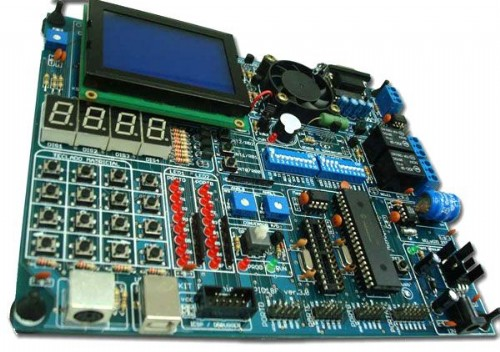
\includegraphics[scale=1]{images/pic_microgenio.png}
 	\caption{Placa Microgenios PIC18F4452}	
 	\label{fig:microgenios}
 	\cite{eletronicabrasil}
 \end{figure}
 
\section{Cálculo por Referência}

Os cálculos do sistema foram todos baseados em número inteiros. Isso devido ao fato de que o uso de ponto flutuante pode causar imprecisões além de consumir mais memória. Para isso toda internamente toda contagem das infusões está em função da quantidade mínima de infusão, 0,1, ou seja, caso seja preciso infundir 1 unidade de insulina internamente o sistema intende como 10. Isso também permite trocar o valor de quantidade minima a ser infundida sem impactar no funcionamento do resto do sistema.

\section{Arquitetura modularizada}

A organização do código é o grande destaque e vantagem desse trabalho. O desacoplamento foi o foco principal durante todo o desenvolvimento isso para facilitar mudanças no próprio \emph{software} ou do \emph{hardware}. 

Esse desacoplamento alcançado deveu-se graças ao uso do conceito OOC, \emph{Object Orientated Programming in ANSI-C}. Através de seu uso pode-se aproveitar das diversas vantagens que a Programação Orientada Objetos proporciona, embora seja um conceito considerado mais volumoso já que seu uso requer um conhecimento de como as linguagens OO abstraem os operadores desse paradigma, pois são implementados manualmente, como:

\begin{itemize}
\item \emph{Bind}: É a associação de uma chamada a um método ou função com sua implementação, de forma mais específica é definir para quem o ponteiro da função está endereçado;
\item Interface: Definição dada por uma \emph{struct} com ponteiros para funções. O \emph{bind} é feito no momento da criação do objeto da classe que implemente essa interface;
\item Classe: Análogo às interfaces, é uma \emph{struct} em que os atributos são ponteiros para função, entretanto tem os \emph{binds} definidos em uma função de criação(construtor) pertencente a essa classe, ou módulo;
\item Construtor: Função da classe responsável por realizar o \emph{bind} de cada ponteiro para cada função da classe, alocações dinâmicas e outras operações que podem ser definidas de acordo com a necessidade de cada classe;
\item Destrutor: Basicamente a liberação de todos os recursos alocados pelo construtor e funções que a classe utilizou;
\item Public: Para declarar um atributo com esse operador de acesso deve-se declarar a variável como atributo da \emph{struct} ou no arquivo header, seja da classe ou da interface;
\item Private: Para esse operador a declaração da variável se dá fora da \emph{struct}, não pode ser no \emph{header}, pois é o arquivo conhecido pelo resto do sistema.
\item Polimorfismo e abstração de dados: Resultado da associação de um mesmo ponteiros de função de uma classe ou interface à funções diferente, variando em função da classe mais especializada que está sendo abstraída.
\end{itemize}

Mas obviamente OOC é limitado e algumas complicações em sua adaptação para o paradigma OO. Validações em tempo de compilação são menos específicas, programação genérica, sintaxe mais complexa, geração de código implícito, entre outros.

Essa abordagem foi importantíssima, pois é possível fazer testes, mocks no sistema, pelo fato de simular programação orientação à objetos, possibilitando realizar testes unitários e utilizando um PC. Uma vez que as classes e interfaces possuem ponteiros de funções, para que o \emph{bind} seja feito nas funções de criação, a realização do mock é muito simples, pois basicamente é fazer com que o ponteiro da função a ser mockada seja endereçada para outra de acordo com o teste a ser realizado. Ao realizar os testes e mocks o acesso aos periféricos, todos os acionamentos e comunicações, ou seja, tudo vinculado ao \emph{hardware} foram redirecionados para um arquivo log de acompanhamento. A definição da arquitetura foi totalmente desenvolvida em função da possibilidade de realização de testes unitários, uma vez que para se realizar os testes é preciso um alto nível de desacoplamento. Os testes foram realizados antes da unificação de todos os módulos do projeto, pois o módulo TimerMotor causou complicações uma vez que não se alcançou o desacoplamento total do \emph{hardware} devido ao \emph{timer} do microcontrolador. A seguir está descrito as vantagens principais de cada módulo devido a forma de implementação.

O módulo Config é o mais simples de todos, sua principal vantagem é o fato de centralizar todas as informações de configuração, fazendo com que o sistema fique mais claro. Além disso, criar casos de testes torna-se simples, pois mudando qualquer uma de suas informações já se reflete no sistema como um todo. É importante lembrar também que ele não carrega nenhuma dependência do compilador ou do hardware, foi implementado em ANSI-C, o que permite que seja utilizado por qualquer compilador e \emph{hardware}.

Os demais módulos foram criados para seguir a ideia de isolação do módulo config. Para isso o que foi feito é deixar as interfaces e funções comuns independente de \emph{hardware} e compilador utilizando apenas ANSI-C. Dessa forma, caso precise de alguma mudança mais drástica relacionada aos dois itens citados o impacto seja mínimo, precisando fazer apenas uma equivalência das funcionalidades específicas. 

Tendo dito as vantagens com relação à mudanças \emph{hardware} e compilador é importante lembrar que a expansibilidade e manutenibilidade do software ficou incrivelmente simples. A ideia foi deixar o "motor" ou "coração" da bomba ter conhecimento apenas das "interface" do sistemas. Dessa forma os detalhes de funcionamento, requisitos de segurança, configurações específicas de hardware para controle dos periféricos e outros, podem ser modificadas sem impactar o funcionamento básico da bomba de infusão. O mais importante é que essas alterações são parametrizáveis, localizando-se no módulo config, e o software sabe quais objetos utilizar e de onde recuperá-los, em algum \emph{Factory} na maioria dos casos. Devido a isso tudo é possível manter mais de um produto em um único código e mudanças importantes no \emph{core} do sistema não precisa ser replicadas e correr risco de conflito entre projetos. Graças ao uso do OOC para criar algo novo basta implementar as funções da interface do módulo em questão e adicionar ao \emph{factory}, caso exista. Segue uma breve explicação do que pode ser feito em cada módulo.

O módulo InsulinPump, responsável por abstrair particularidades de funcionalidades e segurança da bomba para o resto do ambiente, permite criar diversos tipos de bomba. Essa criação leva em conta mudanças nos dois itens citados, por exemplo, bomba europeia, americana, brasileira, que podem ter requisitos de segurança e funcionalidades distintas.

O módulo LCD, responsável por abstrair a forma de uso e qual \emph{display} está sendo utilizado. Ele permite a troca do tipo de LCD utilizado seja simples, por exemplo, trocar o utiliza 2x16, por um 2x12.

O módulo Menu, lembra uma máquina de estado, pois retorna um próximo Menu(estado) ou ele mesmo caso a mudança não seja necessária. Para adicionar um novo menu basta colocá-lo como retorno em alguma situação dentro da função de análise de botões que todos os Menus possuem.

O módulo Motor segue a mesma linha do LCD, permite a troca do periférico por outro motor de passo ou até mesmo um outro tipo de motor. Esse módulo possui um \emph{factory} para que seja possível recuperar o objeto de abstração do motor desejado.

Por fim, o módulo TimerMotor foi criado para desvincular o \emph{timer} que é extremamente dependente do \emph{hardware} e compilador. Foi o módulo mais complicado de se isolar e é o único que não está totalmente isolado devido a algumas limitações da execução de interrupções.